\documentclass[xcolor=dvipsnames,10pt]{beamer}
\usepackage[utf8]{inputenc}
\usepackage[T1]{fontenc}
\usepackage[brazilian]{babel}
\usepackage{etoolbox}
\usepackage{graphicx}
\usepackage{ragged2e}
\usepackage{tikz}

\makeatletter
\patchcmd{\beamer@sectionintoc}{\vskip1.5em}{\vskip0.5em}{}{}
\makeatother

\usefonttheme[professional]{serif}

\justifying

%----------------------------------------------------------------------------------------------------------------------------------

% JUSTIFICAR TEXTO DAS LISTAS DE ITENS

\makeatletter
\renewcommand{\itemize}[1][]{%
  \beamer@ifempty{#1}{}{\def\beamer@defaultospec{#1}}%
  \ifnum \@itemdepth >2\relax\@toodeep\else
    \advance\@itemdepth\@ne
    \beamer@computepref\@itemdepth% sets \beameritemnestingprefix
    \usebeamerfont{itemize/enumerate \beameritemnestingprefix body}%
    \usebeamercolor[fg]{itemize/enumerate \beameritemnestingprefix body}%
    \usebeamertemplate{itemize/enumerate \beameritemnestingprefix body begin}%
    \list
      {\usebeamertemplate{itemize \beameritemnestingprefix item}}
      {\def\makelabel##1{%
          {%
            \hss\llap{{%
                \usebeamerfont*{itemize \beameritemnestingprefix item}%
                \usebeamercolor[fg]{itemize \beameritemnestingprefix item}##1}}%
          }%
        }%
      }
  \fi%
  \beamer@cramped%
  \justifying% NEW
  %\raggedright% ORIGINAL
  \beamer@firstlineitemizeunskip%
}
\makeatother

%%%%%%%%%%%%%%%%%%%%%%%%%%%%
%%TAMANHO DE BLOCOS VARIÁVEIS
\newenvironment<>{varblock}[2][1.2\textwidth]{%
  \setlength{\textwidth}{#1}
  \begin{actionenv}#3%
    \def\insertblocktitle{#2}%
    \par%
    \usebeamertemplate{block begin}}
  {\par%
    \usebeamertemplate{block end}%
  \end{actionenv}}
%%-------------------------
%%%%%%%%%%%%%%%%%%%%%%%%%%%%%%%%%%%%%%%%%%%%%%%%%%%%%%%%%%%%%%%%%%%%%%%%%%%%%%%%
%COR DO TEMPLATE SEMELHANTE AO LOGO
%%%%%%%%%%%%%%%%%%%%%%%%%%%%%%%%%%%%%%%%%%%%%%%%%%%%%%%%%%%%%%%%%%%%%%%%%%%%%%%%
\definecolor{laranja}{rgb}{0.95703125,0.5859375,0.30859375}

%%%%%%%%%%%%%%%%%%%%%%%%%%%%%%%%%%%%%%%%%%%%%%%%%%%%%%%%%%%%%%%%%%%%%%%%%%%%%%%%
%CORES E ESTRUTURAS DE ELEMENTOS DIVERSOS
%%%%%%%%%%%%%%%%%%%%%%%%%%%%%%%%%%%%%%%%%%%%%%%%%%%%%%%%%%%%%%%%%%%%%%%%%%%%%%%%
\setbeamercolor{frametitle}{fg=black}
\setbeamercolor{headline}{fg=black}
\setbeamercolor{footline}{fg=black}
\setbeamercolor{block body}{use=structure,bg=white}
\setbeamercolor{block title}{use=structure,bg=laranja,fg=black}
\setbeamercolor{item}{fg=laranja}
\setbeamercolor{alerted text}{fg=laranja}
\setbeamercolor{section in toc}{fg=black}
\setbeamercolor{title}{fg=black}
\setbeamercolor{subtitle}{fg=black}
\setbeamertemplate{blocks}[rounded][shadow=true]

%%%%%%%%%%%%%%%%%%%%%%%%%%%%%%%%%%%%%%%%%%%%%%%%%%%%%%%%%%%%%%%%%%%%%%%%%%%%%%%%
%PROPRIEDADES VISUAIS DE ELEMENTOS DIVERSOS
%%%%%%%%%%%%%%%%%%%%%%%%%%%%%%%%%%%%%%%%%%%%%%%%%%%%%%%%%%%%%%%%%%%%%%%%%%%%%%%%
\useoutertheme[]{default}
\addtobeamertemplate{block begin}{}{\justifying} % Justify all blocks

\setbeamertemplate{section in toc}[circle]
\setbeamertemplate{subsection in toc}[square]
\setbeamertemplate{itemize item}{$\bullet$}
\setbeamertemplate{navigation symbols}{}
\setbeamercovered{invisible}
\setbeamertemplate{sections in toc}[ball]

%%%%%%%%%%%%%%%%%%%%%%%%%%%%%%%%%%%%%%%%%%%%%%%%%%%%%%%%%%%%%%%%%%%%%%%%%%%%%%%%
%LOGOS POSICIONADOS NO RODAPÉ
%%%%%%%%%%%%%%%%%%%%%%%%%%%%%%%%%%%%%%%%%%%%%%%%%%%%%%%%%%%%%%%%%%%%%%%%%%%%%%%%
\setbeamertemplate{footline}{
  \vspace{0.5em}
  \tikz \fill [laranja] (0,0) rectangle (15, 2pt);

\vspace{-1.3em}
\begin{center}

\includegraphics[height=0.5cm]{logo-iff.png}\hspace{0.4em}

\includegraphics[height=0.5cm]{logo-iprj.png}\hspace{0.4em}

\includegraphics[height=0.5cm]{logo-uerj.png}\hspace{0.4em}

\includegraphics[height=0.5cm]{logo-uesc.png}\hspace{0.4em}

\includegraphics[height=0.5cm]{logo-capes.png}\hspace{0.4em}

\includegraphics[height=0.5cm]{logo-cnpq.png}\hspace{0.4em}

\includegraphics[height=0.5cm]{logo-faperj.png}\hspace{0.4em}

\includegraphics[height=0.5cm]{logo-buzios.png}\vspace{-0.5em}
\end{center}
}

%%%%%%%%%%%%%%%%%%%%%%%%%%%%%%%%%%%%%%%%%%%%%%%%%%%%%%%%%%%%%%%%%%%%%%%%%%%%%%%%
%LOGO DO EVENTO COMO TÍTULO DE TODOS OS SLIDES
%%%%%%%%%%%%%%%%%%%%%%%%%%%%%%%%%%%%%%%%%%%%%%%%%%%%%%%%%%%%%%%%%%%%%%%%%%%%%%%%
\setbeamertemplate{headline}{

\vspace{-1em}
\begin{center}

\includegraphics[width=0.5\textwidth]{logo-evento.png}
\end{center}
}
%%%%%%%%%%%%%%%%%%%%%%%%%%%%%%%%%%%%%%%%%%%%%%%%%%%%%%%%%%%%%%%%%%%%%%%%%%%%%%%%
% INICIO DOS SLIDES
%%%%%%%%%%%%%%%%%%%%%%%%%%%%%%%%%%%%%%%%%%%%%%%%%%%%%%%%%%%%%%%%%%%%%%%%%%%%%%%%
\title{\textbf{\small COMPARISON BETWEEN DIFFERENCIAL EVOLUTION AND SIMULATED ANNEALING ALGORITHMS APPLIED TO THE CONSTRUCTAL DESIGN OF THE DOUBLE-T SHAPED CAVITIES
}}

\author{\small G. V. Gonzales,  L. A. Isoldi, L. A. O. Rocha, E. D. dos Santos e \\
A. J. Silva Neto}
\institute{\vspace{-0.3cm}\scriptsize Programa de Pós-Graduação em Modelagem Computacional - FURG}
%%\subtitle{\vspace{0.3cm}\small Métodos Computacionais\vspace{-0.3cm}}
\date{\vspace{-0.8cm}\scriptsize Outubro de 2018}
\begin{document}

\frame{\titlepage}
\frame{\tableofcontents}

\section{Introdução}
\subsection{Motivação}
\begin{frame}{}
	\begin{block}{\textbf{\textsc{MOTIVAÇÃO}}}
	\justifying
	\setlength{\parindent}{1cm}
	Com a miniaturização dos circuitos eletrônicos e desenvolvimento de dispositivos cada vez mais compactos, técnicas tradicionais de troca térmica por convecção forçada não são mais suportadas. Alternativas apontam para cavidades ou caminhos com material de alta condutibilidade.
	\end{block}
\end{frame}
\subsection{Objetivos}
\begin{frame}{}
	\begin{block}{\textbf{\textsc{OBJETIVOS}}}
	\justifying
	\setlength{\parindent}{1cm}
		\begin{itemize}
		\item Otimizar parcialmente uma cavidade em forma de Duplo-T;
		\item Comparar os resultados de duas meta-heurísticas aplicadas ao problema
		\item Analisar diferentes parâmetros de cada algoritmo;
		\item Avaliar estatisticamente as diferenças entre os resultados da reprodução dos efeitos dos graus de liberdade sobre a geometria ótima e a temperatura máxima minimizada;
		\item Recomendar não só o algoritmo mas também a configuração de parâmetros mais adequada ao problema de otimização;
	\end{itemize}
	\end{block}
\end{frame}

\subsection{Breve Estado da Arte}
	\begin{frame}{}
	\begin{block}{\textbf{\textsc{BREVE ESTADO DA ARTE}}}	
\justifying
	\setlength{\parindent}{1cm}
		\begin{itemize}
		\item Cavidade em formato de "C" e "T"  em Biserni et. al. (2004). 
		\item Cavidade em forma de "H"  em Biserni et. al.(2007).
		\item Cavidade em forma de "Y"  em (Lorenzini et. al.(2011).
		\item Cavidade em forma de "Y" aplicação do Algoritmo Genético  em Lorenzini et. al.(2014).
		\item Comparação entre aplicação do SA com GA na otimização da cavidade em forma de Y  em Gonzales et. al.(2015a).
		\item Otimização parcial até 3 graus de liberdade da cavidade em duplo-T  em Gonzales et. al. (2015b).
	\end{itemize}
	\end{block}
\end{frame}

\section{Modelagem Matemática e Numérica}

\begin{frame}[plain]
\begin{block}{\textbf{MODELAGEM MATEMÁTICA E NUMÉRICA}}
\begin{figure}[h!]
			\centering
			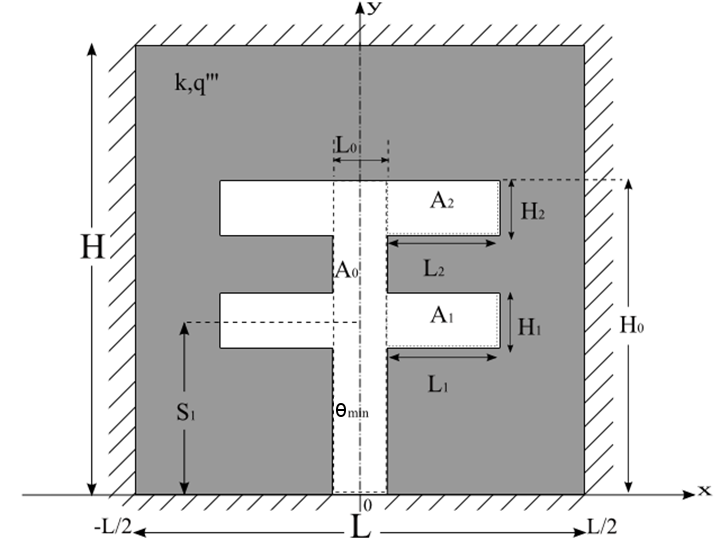
\includegraphics[width=0.9\linewidth]{../../imgs/duplo_t.png}
			\caption{ {\small Domínio Computacional da Cavidade em Forma de Duplo-T.}}
			\label{figure01}
		\end{figure}
\end{block}
\end{frame}


\begin{frame}{}
\begin{block}{\textbf{\textsc{MODELAGEM MATEMÁTICA E NUMÉRICA}}}
\justifying
	\setlength{\parindent}{1cm}
		\textbf{Hipóteses Simplificativas:}
		\small
		\begin{enumerate}
			\item Regime Permanente
			\item Geração uniforme de calor
			\item Condutividade térmica constante
			\item Domínio bidimensional
		\end{enumerate}
		\normalsize
		\begin{equation}
		\frac{\partial}{\partial x}\left( k\frac{\partial \theta}{\partial x}\right)+
		\frac{\partial}{\partial y}\left(k\frac{\partial \theta}{\partial y}\right)+
		\frac{\partial}{\partial z}\left(k\frac{\partial \theta}{\partial z}\right)+ 
		q^{'''}=\rho C_p\frac{\partial \theta}{\partial t}\label{calor}
		\end{equation}
		\begin{equation}
		\frac{\partial ^{2} \theta}{\partial x^{2}}+\frac{\partial ^{2} \theta}{\partial y^{2}}+\frac{q^{'''}}{k}=0\label{calor}
		\end{equation}
	\end{block} 
\end{frame}

\begin{frame}{}
	\begin{block}{\textbf{\textsc{MODELAGEM MATEMÁTICA E NUMÉRICA}}}
	\textbf{Restrições: }
		\begin{equation}
			A = HL \label{area_total}
		\end{equation}
		\begin{equation}
			A_{c} = A_{0} + 2A_{1} + 2A_{2} \label{area_cavidade}
		\end{equation}\begin{equation}
			\phi_{c} = A_{c}/A \label{fi}
		\end{equation}
		
	\end{block} 
\end{frame}


\begin{frame}
\begin{varblock}[11.5cm]{\textbf{\textsc{MODELAGEM MATEMÁTICA E NUMÉRICA}}}\justifying
	\setlength{\parindent}{1cm}
\textbf{Adimensionalização do Problema:}
		\begin{equation}
				\tilde{x},\tilde{y},\tilde{H}_{0},\tilde{H}_{1},\tilde{H}_{2},\tilde{L}_{0},\tilde{L}_{1},\tilde{L}_{2},\tilde{H},\tilde{L},\tilde{S}_{1} = \frac{x,y,H_{0},H_{1},H_{2},L_{0},L_{1},L_{2},H,L,S_{1}}{A^{1/2}}\label{vadim} 
		\end{equation}
		\begin{equation}
				\frac{\partial ^{2}\tilde{\theta}}{\partial \tilde{x}^{2}}+\frac{\partial ^{2} \tilde{\theta}}{\partial \tilde{y}^{2}}+1=0\label{calor}
		\end{equation}
		\begin{equation}
			\tilde{\theta}_{max}=\frac{\theta_{max}-\theta_{min}}{q^{'''}\cdot\frac{A}{k}}\label{fo}
		\end{equation}
		\end{varblock}
\end{frame}
\begin{frame}
\begin{block}{\textbf{\textsc{MODELAGEM MATEMÁTICA E NUMÉRICA}}}
\justifying
	\setlength{\parindent}{1cm}
		A função representada pela Eq. \ref{fo} é resolvida numericamente através da resolução da Eq. \ref{calor} para a determinação dos os campos de temperatura em todo o domínio computacional para diferentes configurações de ($H$, $L$, $H_{0}$, $L_{0}$, $H_{1}$, $L_{1}$, $H_{2}$, $L_{2}$ e $S_{1}$) e calculando o $\tilde{\theta}_{max}$ para minimizar o seu valor através da variação da configuração geométrica.\\ A solução numérica é dada pela aplicação do método de Elementos Finitos (FEM), baseado em elementos triangulares, desenvolvido no ambiente MATLAB$^{\tiny ®}$, com o pacote PDE (partial-differential-equations) toolbox.\\ A malha utilizada é não-uniforme em ambos eixos $x$ e $y$, e varia de uma geometria para outra. O tamanho é de  80649 mil elementos.
	\end{block}
\end{frame}
\section{Otimização}
\begin{frame}
	\begin{block}{\textbf{\textsc{OTIMIZAÇÃO}}}
	\justifying
	\setlength{\parindent}{1cm}
	A metodologia de otimização aplicada neste trabalho utiliza-se do método Constructal Design associado as meta-heurísticas Differential Evolution (DE) e Simulated Annealing (SA). 
	\begin{itemize}
		\item \textbf{Constructal Desing}: para definição dos objetivos, restrições, Graus de Liberdade (GL) e espaço de busca.
		\item \textbf{Algoritmos de Otimização}: neste trabalho aplicamos os algoritmos DE e SA  para a obtenção das geometrias ótimas.
		\item \textbf{Comparação dos Resultados}: São utilzidos os valores de média entre 30 execuções de cada algoritmo e comparados com os melhores resultados encontrados entre todas as rodadas.
	\end{itemize}
	\end{block}
\end{frame}
\subsection{Design Construtal}
\begin{frame}{}
	\begin{block}{\textbf{CONSTRUCTAL DESIGN}}
		\justifying
		\setlength{\parindent}{1cm}
		\textbf{Definição dos Graus de Liberdade e Restrições:}
		\begin{itemize}
			\item Nove variáveis ($H$, $L$, $H_{0}$, $L_{0}$, $H_{1}$, $L_{1}$, $H_{2}$, $L_{2}$ e $S_{1}$);
			\item Quatro restrições ($A$,$A_c$,$A_1$ e $A_2$);
			\begin{equation}
				\phi_c = A_c/A= \tilde{H_{0}}\tilde{L_{0}}+2\phi_1+2\phi_2
			\end{equation}
			\begin{equation}
				\phi_1 = \tilde{H_{1}}\tilde{L_{1}} 
			\end{equation}
			\begin{equation}
				\phi_2 = \tilde{H_{2}}\tilde{L_{2}}
			\end{equation}
			\item Temos cinco Graus de liberdade ($H/L$, $H_{0}/L_{0}$, $H_{1}/L_{1}$, $H_{2}/L_{2}$ e $S_{1}/H_{0}$) para o fechamento das equações;
			
		\end{itemize}
	\end{block}
\end{frame}
\begin{frame}{}
	\begin{block}{\textbf{CONSTRUCTAL DESIGN}}
		\justifying
		\setlength{\parindent}{1cm}
		\begin{itemize}
\item Durante o processo de otimização, foram mantidos constantes os valores das restrições ($\phi_c = 0.1,  \phi_1 = \phi_2 = 0.015$) 
\item Para a otimização de 3 Gls  o grau de liberdade $H_{0}/L_{0}$ foi variado entre $0 =< H_{0}/L_{0}<= 25$;
\item Sendo otimizados os graus de liberdade: $H_{2}/L_{2}$, $H_{1}/L_{1}$ e $S_{1}/H_{0}$;
\item Para a otimização de 4 GLs, o grau de liberdade $H/L$ foi variado entre $0.3 =< H/L<= 30$;
			\item Sendo otimizados os graus de liberdade: $H_{0}/L_{0}$, $H_{1}/L_{1}$, $H_{2}/L_{2}$ e $S_{1}/H_{0}$;
		\end{itemize}
	\end{block}
\end{frame}

\subsection{Configuração dos Algoritmos}
\begin{frame}{}
\begin{block}{
\textbf{\textsc{CONFIGURAÇÃO DOS ALGORITMOS}}}
			\begin{table}[H] % !htbp
			\caption{Versões do Algoritmo Differential Evolution. }
			\label{table1}
			\vspace{5pt}
			\centering{}
			\begin{tabular*}{\textwidth}{@{\extracolsep{\fill}}c|c|c|c|c}        % {0.8\textwidth}
			\hline
				& DE1 & DE2 & DE3 & DE4 \tabularnewline
			\hline
				Amplificação $F$ & 1,5 & 2,0 & 1,5 & 2,0\tabularnewline
			\hline 
				Cruzamento & 0,7 & 0,9 & 0,7 & 0,9\tabularnewline
			\hline
				Mutação & rand/1/bin & rand/1/bin & best/2/bin & best/2/bin \tabularnewline
			\hline 
				Iter. $H_{0}/L_{0}$ & 150 & - & - & -\tabularnewline
			\hline
				Iter $H/L$ & 300 & - & - & - \tabularnewline
			\hline
			\end{tabular*}
			\end{table}
			\end{block}
\end{frame}	
\begin{frame}
\begin{varblock}[11.5cm]{
\textbf{\textsc{CONFIGURAÇÃO DOS ALGORITMOS}}}
			\begin{table}[H] % !htbp
			\caption{Versões do Algoritmo Simulated Annealing. }
			\label{table1}
			\vspace{5pt}
			\centering{}
			\begin{tabular*}{\textwidth}{@{\extracolsep{\fill}}c|c|c|c|c|c} %%{0.8\textwidth}	
			\hline
				& SAEX & SABO & SABE & SAC1 & SAC2\tabularnewline
			\hline
				C. Schedule & \small Exponencial & \small Boltz & \small BoltzExp & \small ConstExp1 &  
\small ConstExp2\tabularnewline
			\hline 
				Iter. $H_{0}/L_{0}$ & 150 & - & - & -&-\tabularnewline
			\hline
				Iter $H/L$ & 300 & - & - & - & -\tabularnewline
			\hline
			\end{tabular*}
			\end{table}				
			\end{varblock}
	\end{frame}


\section{Resultados}

%\begin{frame}
%\begin{block}{\textbf{\textsc{RESULTADOS}}}
%\justifying
%		\setlength{\parindent}{1cm}
%\justifying
%		\setlength{\parindent}{1cm}
%\begin{itemize}
%			\item Primeiramente serão apresentados os resultados da otimização de 3 GLs, com o efeito de $H_{0}/L_{0}$ sobre a geometria ótima ($(H_{2}/L_{2})_{3 \times o}$, $(H_{1}/L_{1})_{2\times o}$ e $(S_{1}/H_{0})_{o}$) e temperatura máxima em excesso três vezes minimizada $(\tilde{\theta}_{max})_{3\times m}$.
%			\item Foram investigados valores de  $H_{0}/L_{0}$ no intervalo de 0 a 25, onde para cada valor foram executadas 30 rodadas de cada algoritmo.
%			
%		\end{itemize}
%\end{block}
%\end{frame}

\begin{frame}[plain]
\begin{block}{\textbf{\textsc{PRINCIPAIS RESULTADOS}}}
\begin{figure}[H]
\centering
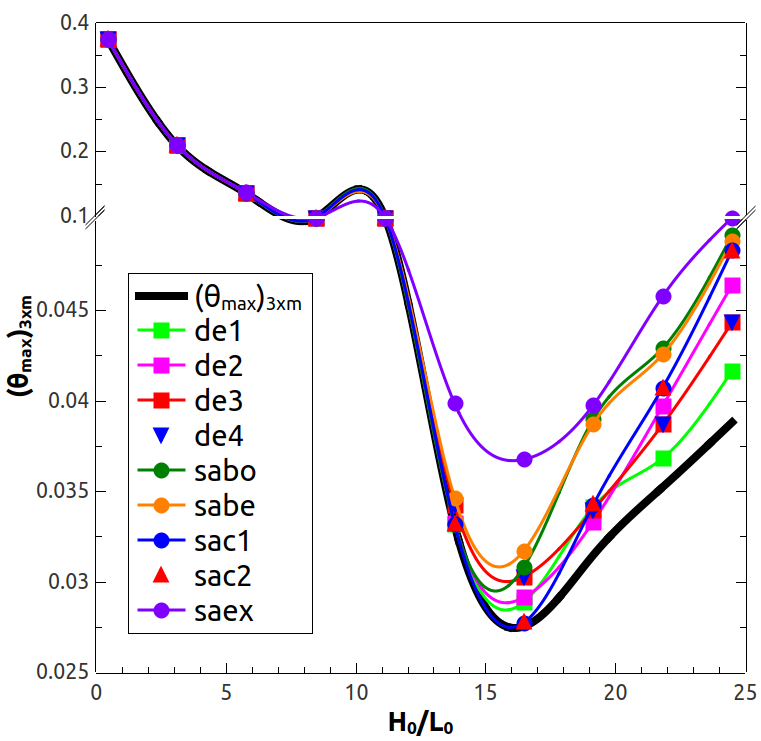
\includegraphics[width=0.65\linewidth]{../../imgs/4dof/h0l0-tmin.png}
\caption{ {\small Efeito de $H_{0}/L_{0}$ sobre $(\tilde{\theta}_{max})_{3\times m}$ obtidos por cada versão dos algoritmos DE e SA.}}
\label{figure02}
\end{figure}
\end{block}
\end{frame}

\begin{frame}[plain]
\begin{block}{\textbf{\textsc{PRINCIPAIS RESULTADOS}}}
\begin{figure}[H]
\centering
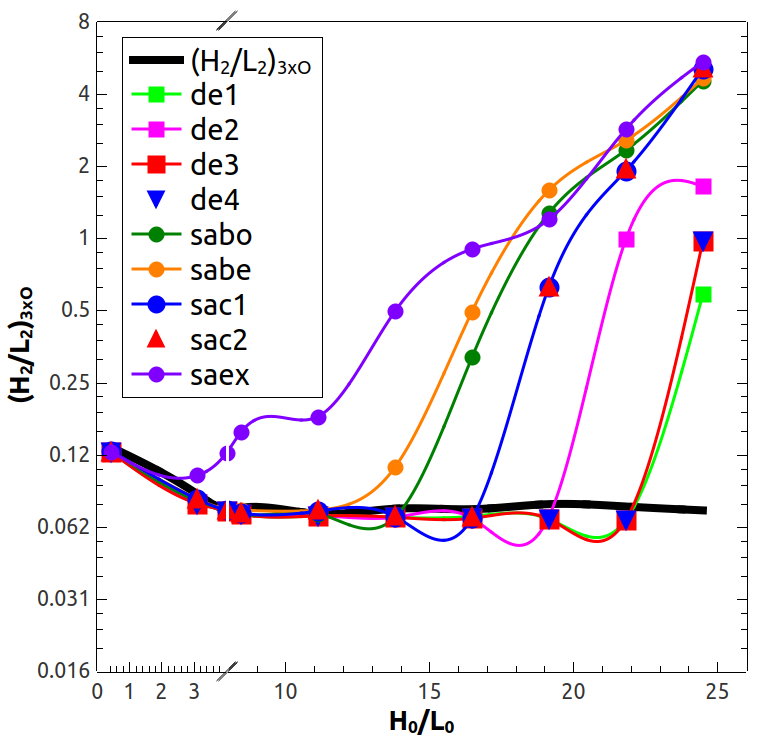
\includegraphics[width=0.65\linewidth]{../../imgs/4dof/h0l0-h2l2.png}
\caption{ {\small Efeito de $H_{0}/L_{0}$ sobre $(H_{2}/L_{2})_{3\times o}$ obtidos por cada versão dos algoritmos DE e SA.}}
\label{figure03}
\end{figure}
\end{block}
\end{frame}


%\begin{frame}[plain]
%\begin{block}{\textbf{\textsc{RESULTADOS}}}
%\begin{figure}[H]
%\centering
%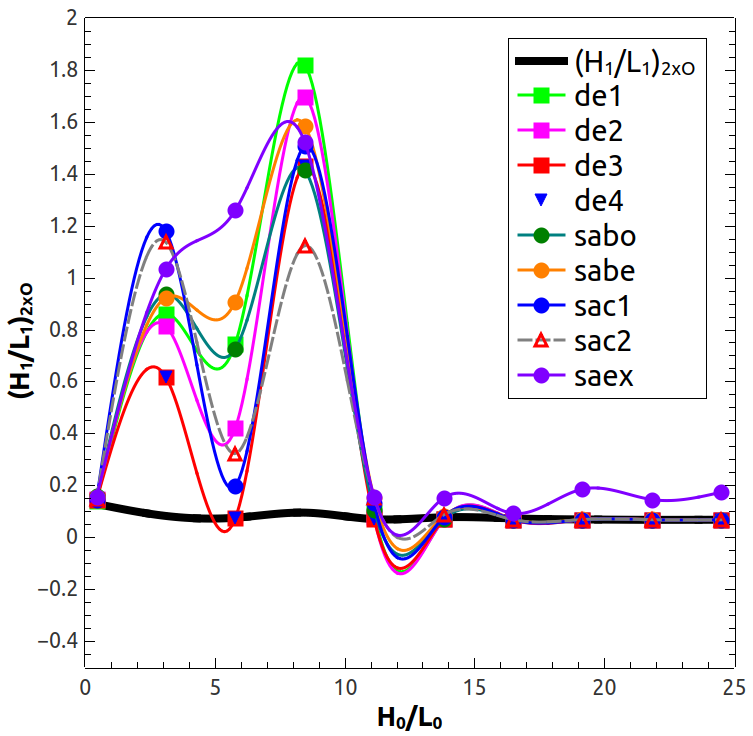
\includegraphics[width=0.65\linewidth]{../../imgs/4dof/h0l0-h1l1.png}
%\caption{ {\small Efeito de $H_{0}/L_{0}$ sobre $(H_{1}/L_{1})_{2\times o}$ obtidos por cada versão dos algoritmos DE e SA.}}
%\label{figure04}
%\end{figure}
%\end{block}
%\end{frame}


%
%\begin{frame}[plain]
%\begin{block}{\textbf{\textsc{RESULTADOS}}}
%\begin{figure}[H]
%\centering
%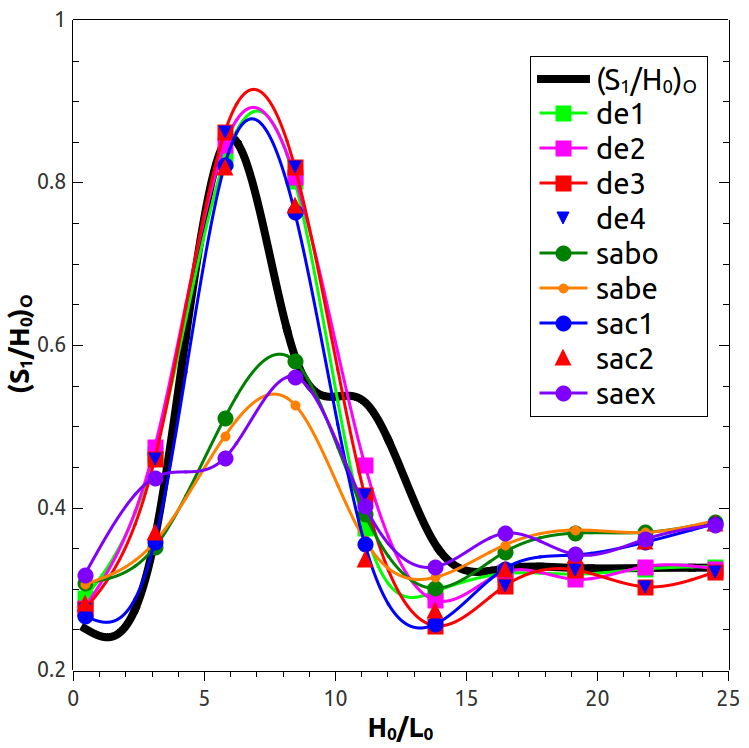
\includegraphics[width=0.65\linewidth]{../../imgs/4dof/h0l0_s1h0.png}
%\caption{ {\small Efeito de $H_{0}/L_{0}$ sobre $(S_{1}/H_{0})_{o}$ obtidos por cada versão dos algoritmos DE e SA.}}
%\label{figure05}
%\end{figure}
%\end{block}
%\end{frame}

%\begin{frame}
%\begin{block}{\textbf{\textsc{RESULTADOS}}}
%\justifying
%		\setlength{\parindent}{1cm}
%\begin{itemize}
%			\item A seguir serão apresentados os resultados para a otimização de 4 Gls para diferentes valores de $H/L$.
%			\item O grau de liberdade $H/L$ foi variado entre os valores 0.3 a 30.
%			
%		\end{itemize}
%\end{block}
%\end{frame}

\begin{frame}[plain]
\begin{varblock}[11.5cm]{\textbf{\textsc{PRINCIPAIS RESULTADOS}}}
\begin{figure}[H]
\centering
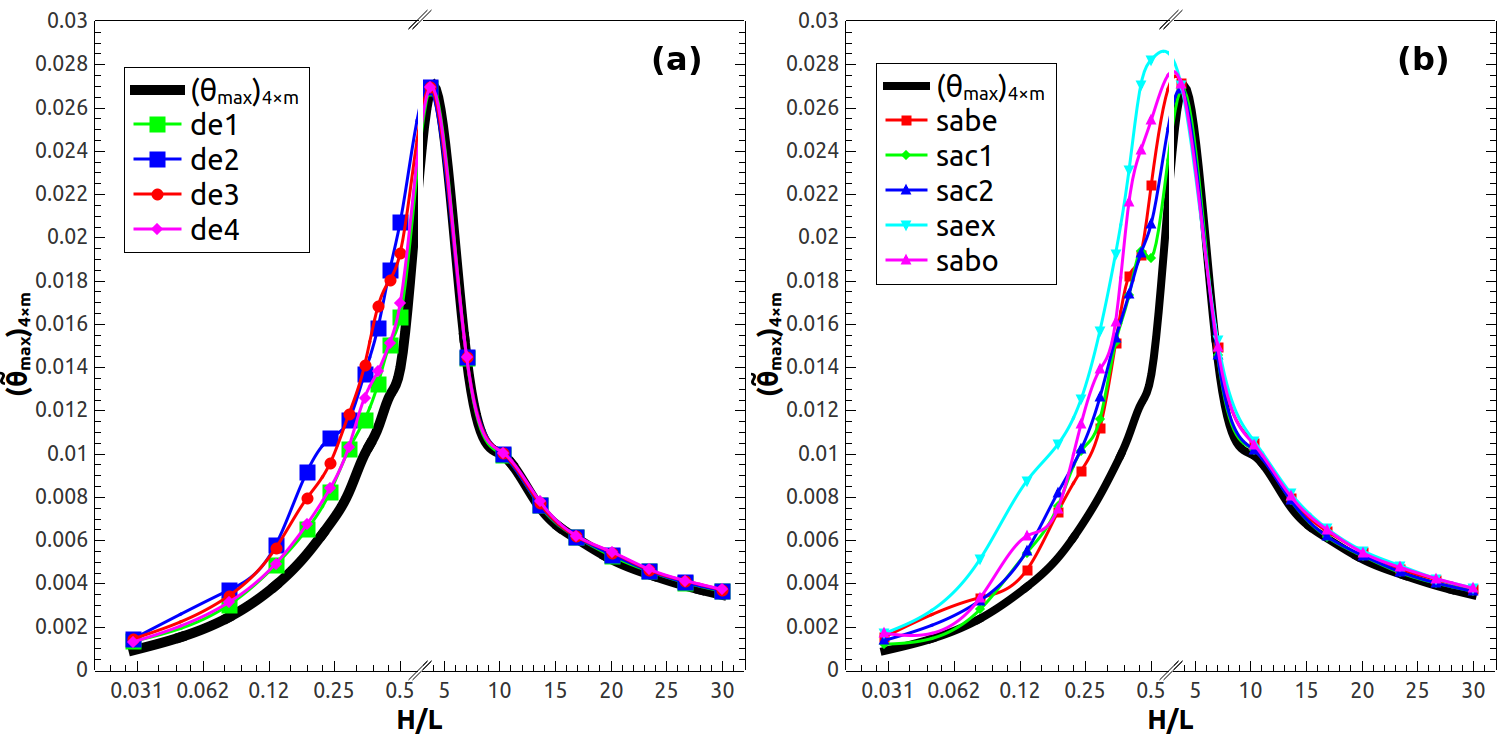
\includegraphics[width=1.01\linewidth]{../../imgs/5dof/de_sa_hl_tmin.png}
\caption{ {\small Efeito de $H/L$ sobre $(\tilde{\theta}_{max})_{3\times m}$ obtidos por cada versão dos algoritmos DE e SA: a) DE b) SA}}
\label{figure06}
\end{figure}
\end{varblock}
\end{frame}

%\begin{frame}[plain]
%\begin{varblock}[11.5cm]{\textbf{\textsc{RESULTADOS}}}
%\begin{figure}[H]
%\centering
%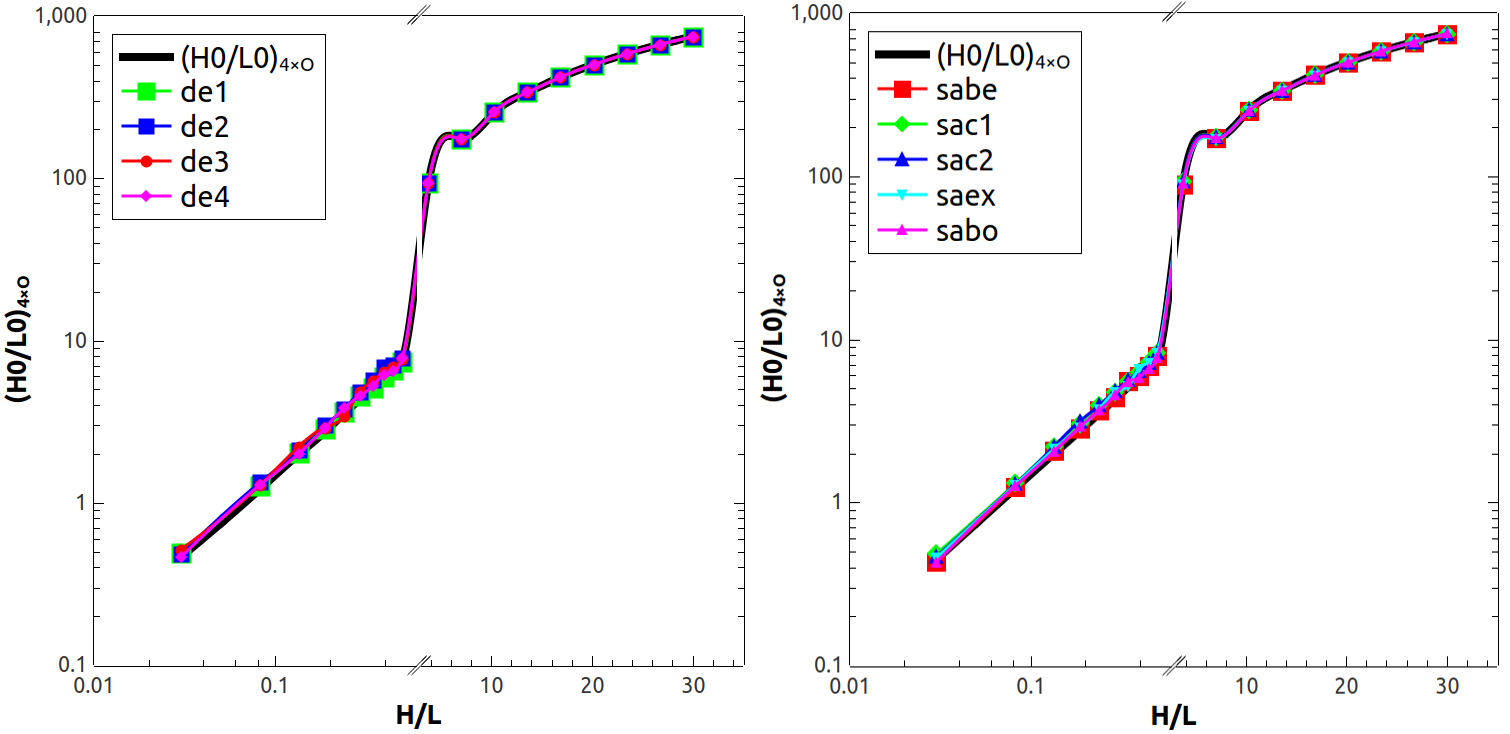
\includegraphics[width=1.01\linewidth]{../../imgs/5dof/de_sa_hl_h0l0.png}
%\caption{ {\small Efeito de $H/L$ sobre $(H_{0}/L_{0})_{4\times o}$ obtidos por cada versão dos algoritmos DE e SA: a) DE b) SA}}
%\label{figure07}
%\end{figure}
%\end{varblock}
%\end{frame}

\begin{frame}[plain]
\begin{varblock}[11.5cm]{\textbf{\textsc{PRINCIPAIS RESULTADOS}}}
\begin{figure}[H]
\centering
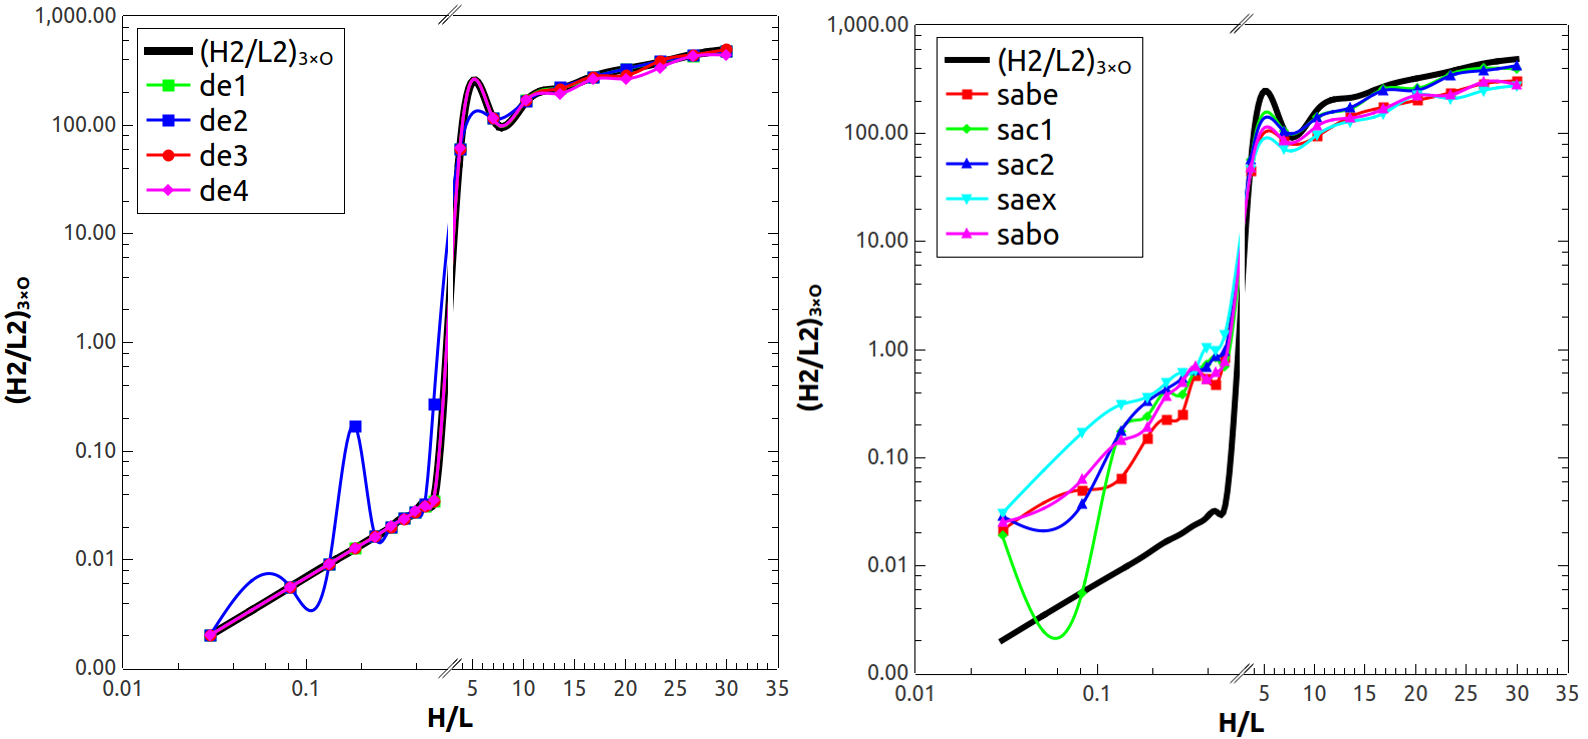
\includegraphics[width=1.01\linewidth]{../../imgs/5dof/de_sa_hl_h2l2.png}
\caption{ {\small Efeito de $H/L$ sobre $(H_{2}/L_{2})_{3\times o}$ obtidos por cada versão dos algoritmos DE e SA: a) DE b) SA}}
\label{figure08}
\end{figure}
\end{varblock}
\end{frame}

\begin{frame}[plain]
\begin{varblock}[11.5cm]{\textbf{\textsc{PRINCIPAIS RESULTADOS}}}
\begin{figure}[H]
\centering
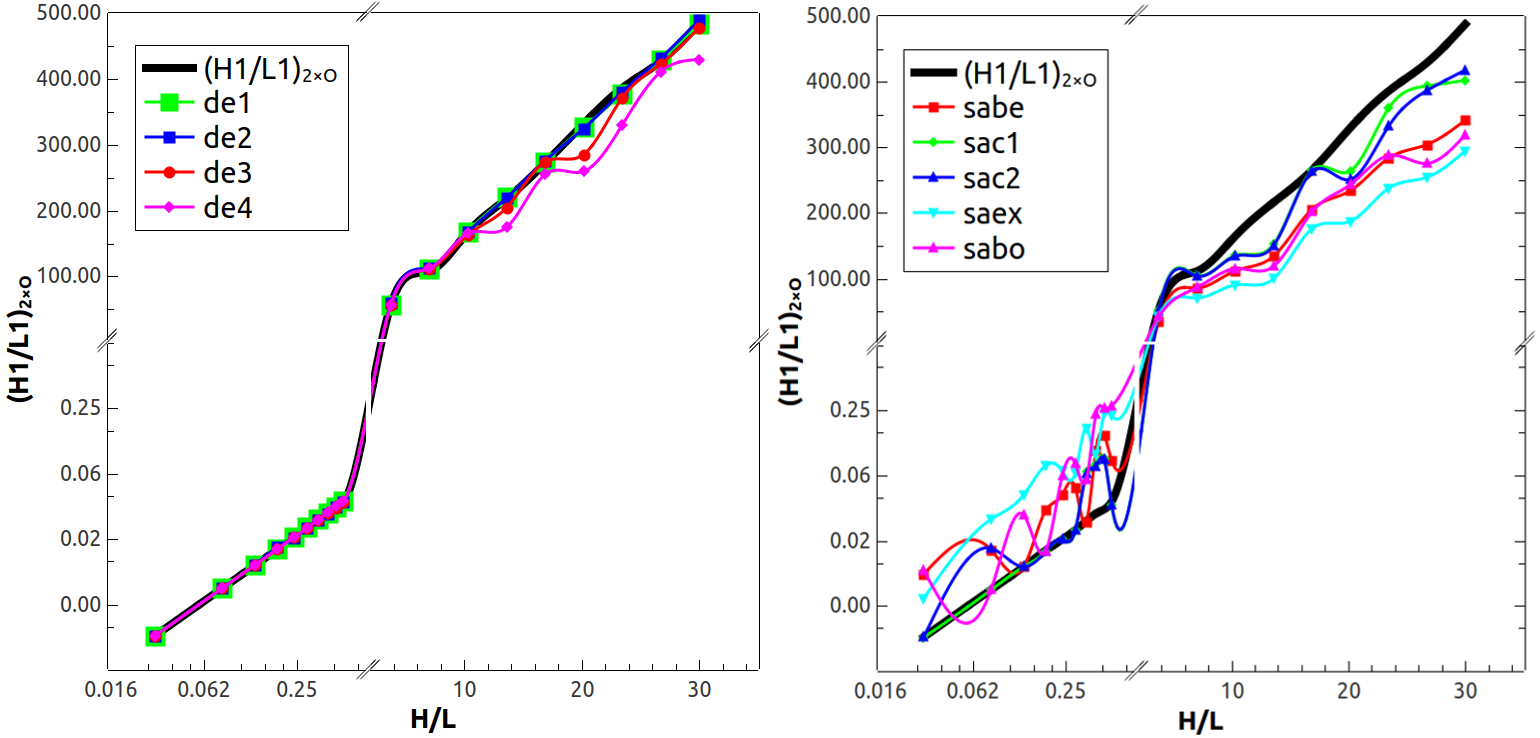
\includegraphics[width=1.01\linewidth]{../../imgs/5dof/de_sa_hl_h1l1.png}
\caption{ {\small Efeito de $H/L$ sobre $(H_{1}/L_{1})_{2\times o}$ obtidos por cada versão dos algoritmos DE e SA: a) DE b) SA}}
\label{figure11}
\end{figure}
\end{varblock}
\end{frame}

%\begin{frame}[plain]
%\begin{varblock}[11.5cm]{\textbf{\textsc{RESULTADOS}}}
%\begin{figure}[H]
%\centering
%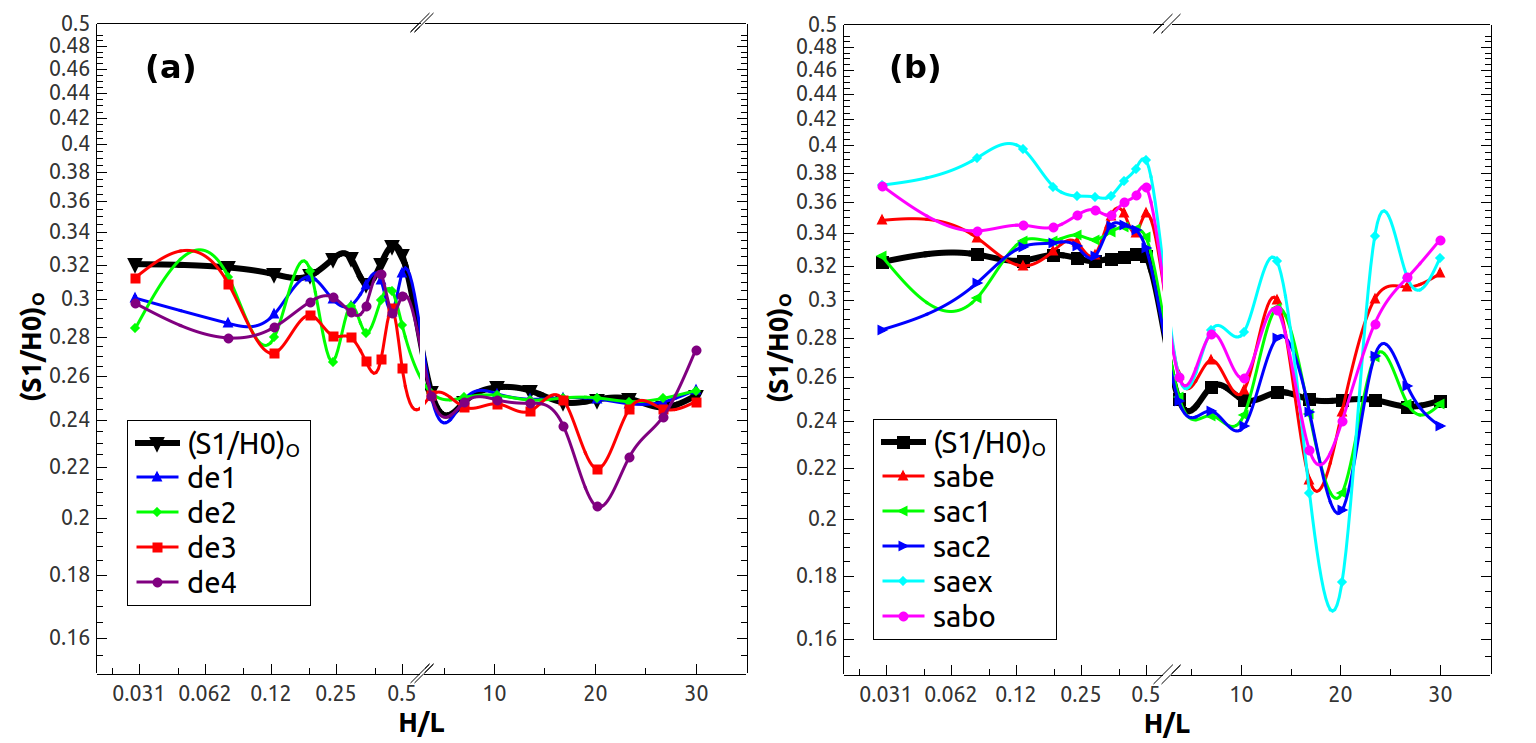
\includegraphics[width=1.01\linewidth]{../../imgs/5dof/de_sa_hl_s1h0.png}
%\caption{ {\small Efeito de $H/L$ sobre $(S_{1}/H_{0})_{o}$ obtidos por cada versão dos algoritmos DE e SA: a) DE b) SA}}
%\label{figure12}
%\end{figure}
%\end{varblock}
%\end{frame}

\section{Conclusão}

%\begin{frame}
%\begin{block}{\textbf{\textsc{CONCLUSÃO}}}
%\justifying
%		\setlength{\parindent}{1cm}
%		\begin{itemize}
%			\item O trabalho analisou os resultados de duas meta-heurísticas aplicadas a otimização geometrica em um problema de transferência de calor. 
%			\item O objetivo principal é encontrar o algoritmo com os melhores resultados para a reprodução do efeito dos graus de liberdade sobre a geometria ótima e a performance térmica do problema
%			\item Foi observado que a meta-heurística empregada pode levar a interpretações erradas em relação a influência de um grau de liberdade sobre a configuração ótima. Reproduzindo curvas de efeito imprecisas.
%			
%		\end{itemize}
%\end{block}
%\end{frame}

\begin{frame}
\begin{block}{\textbf{\textsc{CONCLUSÃO}}}
\justifying
		\setlength{\parindent}{1cm}
		\begin{itemize}
			\item Dentre os algoritmos pesquisados e as configurações de parâmetros avaliadas, todas as versões do SA apresentaram um desempenho inferior as versões do DE.
			\item O DE foi o que apresentou, em geral, melhor desempenho. Principalmente as versões DE1 e DE4, com os parâmetros de cruzamento de 0.9 e fator de amplificação de 1.5;
			\item Portanto, para o problema de interesse, esses são os parâmetros recomendados para o algoritmo DE, pois foram aqueles que reproduziram de maneira mais precia as curvas de efeito dos graus de liberdade sobre a geometria ótima e peformance térmica do problema. 
		\end{itemize}
\end{block}
\end{frame}

\section{Referências}

\begin{frame}

\begin{block}{\textbf{\textsc{REFERÊNCIAS}}}
\begin{thebibliography}{99}
\fontsize{8}{0}\selectfont

\bibitem[Bejan, 1996]{Bejan}
A. Bejan, Constructal-theory Network of Conducting Path for Cooling a Heat Generating Volume. {\it Int. J. Heat Mass Transfer}, vol. 40, n. 4, pp.799-816, 1996.

\bibitem[Biserni et al., 20104]{Biserni1}
C. Biserni, L. A. O. Rocha, A. Bejan, Inverted Fins: Geometric Optimization of the Intrusion Into a Conducting Wall. {\it Int. J. Heat and Mass Transfer}, 47, pp. 2577-2586, 2004.

\bibitem[Gonzales et al., 2015]{Gonzales2}
G. V. Gonzales, E. D. Dos Santos, L. A. Isoldi, E. da S. D. Estrada,L. A. O. Rocha, Constructal Design of Isothermal Double-T Shaped Cavity By Means of Simulated Annealing. In {\it Proceedings of the XXXVI Iberian Latin-American Congress on Computational Methods in Engineering}, Rio de Janeiro, RJ, Brazil, 2015.

\bibitem[Kirkpatrick et al.,1983]{Kirk}
S. Kirkpatrick, C. D. Gelatt, M. P. Vecchi, M. P., Optimization by Simulated Annealing. {\it Science}, New Series., v. 220, No 4598, pp 671-680, 1983.
\end{thebibliography}
\end{block}
\end{frame}

\begin{frame}
\begin{block}{\textbf{\textsc{REFERÊNCIAS}}}
\begin{thebibliography}{99}
\fontsize{8}{0}\selectfont

\bibitem[Lorenzini et al., 2014]{Lorenzini4}
G. Lorenzini, C. Biserni, E. da S. D. Estrada, E. D. Dos Santos, L. A. Isoldi, L. A. O. Rocha, Genetic Algorithm Applied to Geometric Optimization of Isothermal Y-Shaped Cavities. {\it Journal of Electronic Packaging }, vol 136, p. 031011-031011-9, 2014.

\bibitem[Metropolis et al.,1953]{Metropolis}
N. Metropolis, A. W. Rosenbluth, M. N. Rosenbluth, A. H. Teller, E. Teller, Equation of State Calculations by Fast Computing Machines. {\it The Journal of Chemical Physics.}, v 21, p 1088-1092, 1953.

\bibitem[Storn and Price., 1997]{Storn}
R. Storn, K. Price, Differential Evolution - A Simple and Efficient Heuristic for Global Optimization over Continuous Spaces. {\it Journal of Global Optimization.}, v 11, p 341-359, 1997.

\end{thebibliography}
\end{block}
\end{frame}

\section{Agradecimentos}
\begin{frame}
\begin{block}{\textbf{\textsc{AGRADECIMENTOS}}}
\begin{figure}[h!]
			\centering
			
\includegraphics[width=0.8\linewidth]{../../imgs/agrade.png}
			\label{figure01}
	\end{figure}
\end{block}
\end{frame}

\end{document}